\documentclass[landscape]{article}
\usepackage[dvipsnames]{xcolor}
\usepackage{tikz}

\usetikzlibrary{patterns,snakes}
\usepackage{stackengine}

\begin{document}


\begin{center}
  \hspace{-3.0in}
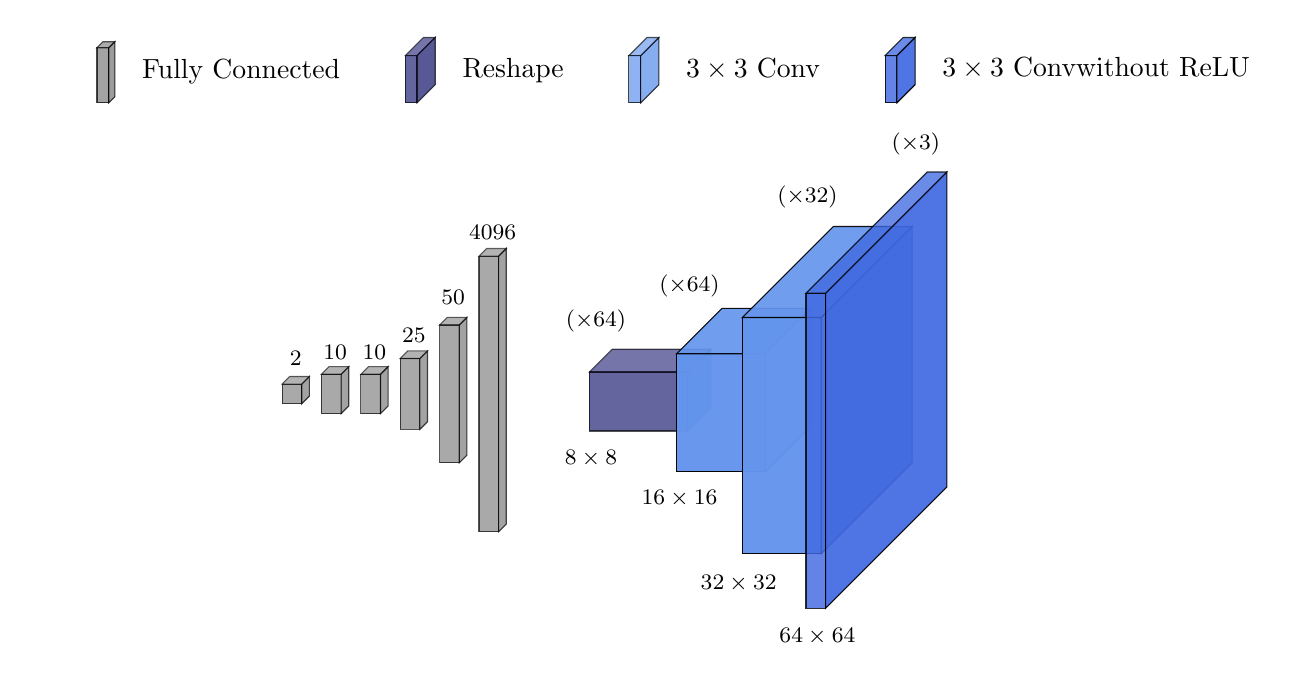
\begin{tikzpicture}[scale=0.5]
  %%%%%%%%%%%%%%%%%%%%%%%%%%%%%%%%%%%%%%%%%%%%%%%%%%%%%%%%%%%%%%%%%%%%%%%%%%%%%%%%%%%%%%%%%%%%%%%%%%%%%%%%%%%%%%%%%%%%%%%%%%
  %%%  PARAMETERS:
  %%%%%%%%%%%%%%%%%%%%%%%%%%%%%%%%%%%%%%%%%%%%%%%%%%%%%%%%%%%%%%%%%%%%%%%%%%%%%%%%%%%%%%%%%%%%%%%%%%%%%%%%%%%%%%%%%%%%%%%%%%

  
  %%% COLOR PALLETE %%%
  \def\colora{CornflowerBlue}
  \def\colorb{Gray}
  \def\colorf{MidnightBlue}
  \def\colorg{RoyalBlue}
  
  %%% CENTER X-Y COORDINATES
  \def\cx{0}
  \def\cy{0}

  %%% FRONT/SIDE/TOP OPACITIES
  %\def\fopac{0.875}
  %\def\sopac{0.925}
  %\def\topac{0.8}
  \def\fopac{0.975}
  \def\sopac{0.875}
  \def\topac{0.925}

  \def\fopacb{0.675}
  \def\sopacb{0.725}
  \def\topacb{0.6}

  \def\fopacc{0.825}
  \def\sopacc{0.925}
  \def\topacc{0.775}


  %%%%%%%%%%%%%%%%%%%%%%%%%%%%
  %%% LEGEND
  %%%%%%%%%%%%%%%%%%%%%%%%%%%%

  %%% CENTER X-Y COORDINATES
  \def\cx{0}
  \def\cy{0}

  \node at (6.75,8) {
    \setlength\tabcolsep{1.5pt}
    \begin{tabular}{clclcl}
      \def\depth{0.15}
      \def\res{0.35}
      \def\resalt{0.1}
      \def\initd{0}
      \def\fcolor{\colorb}
      \tikz{\draw[fill=\fcolor,opacity=0.725] (\initd,\cx-\res,\cy+\resalt) -- ++(\depth,0,0) -- ++(0,2*\res,0) -- ++(-\depth,0,0) -- cycle;
      \draw[fill=\fcolor,opacity=0.775] (\initd+\depth,\cx-\res,\cy+\resalt) -- ++(0,0,-2*\resalt) -- ++(0,2*\res,0) -- ++(0,0,2*\resalt) -- cycle;
      \draw[fill=\fcolor,opacity=0.65] (\initd,\cx+\res,\cy+\resalt) -- ++(\depth,0,0) -- ++(0,0,-2*\resalt) -- ++(-\depth,0,0) -- cycle;}
      & \raisebox{0.125in}{ \hspace{0.0in} Fully Connected} \hspace{0.0in} 
      %%%%%%%%%%%%%%%%%%%%%%%%%%%%%%%%%%%%%%%%%%%%%%%%%%%%%%%%%%%%%%%%%%%%%%%%%%%
      \def\depth{0.15}
      \def\res{0.3}
      \def\resalt{0.3}
      \def\initd{0}
      \def\fcolor{\colorf}
      \tikz{\draw[fill=\fcolor,opacity=\fopacb] (\initd,\cx-\res,\cy+\resalt) -- ++(\depth,0,0) -- ++(0,2*\res,0) -- ++(-\depth,0,0) -- cycle;
      \draw[fill=\fcolor,opacity=\sopacb] (\initd+\depth,\cx-\res,\cy+\resalt) -- ++(0,0,-2*\resalt) -- ++(0,2*\res,0) -- ++(0,0,2*\resalt) -- cycle;
      \draw[fill=\fcolor,opacity=\topacb] (\initd,\cx+\res,\cy+\resalt) -- ++(\depth,0,0) -- ++(0,0,-2*\resalt) -- ++(-\depth,0,0) -- cycle;}
      & \raisebox{0.13in}{ \hspace{0.0in} Reshape} \hspace{0.0in} 
      %%%%%%%%%%%%%%%%%%%%%%%%%%%%%%%%%%%%%%%%%%%%%%%%%%%%%%%%%%%%%%%%%%%%%%%%%%%
      %%%%%%%%%%%%%%%%%%%%%%%%%%%%%%%%%%%%%%%%%%%%%%%%%%%%%%%%%%%%%%%%%%%%%%%%%%%
      \def\depth{0.15}
      \def\res{0.3}
      \def\resalt{0.3}
      \def\initd{0}
      \def\fcolor{\colora}
      \tikz{\draw[fill=\fcolor,opacity=0.725] (\initd,\cx-\res,\cy+\resalt) -- ++(\depth,0,0) -- ++(0,2*\res,0) -- ++(-\depth,0,0) -- cycle;
      \draw[fill=\fcolor,opacity=0.775] (\initd+\depth,\cx-\res,\cy+\resalt) -- ++(0,0,-2*\resalt) -- ++(0,2*\res,0) -- ++(0,0,2*\resalt) -- cycle;
      \draw[fill=\fcolor,opacity=0.65] (\initd,\cx+\res,\cy+\resalt) -- ++(\depth,0,0) -- ++(0,0,-2*\resalt) -- ++(-\depth,0,0) -- cycle;}
      & \raisebox{0.13in}{ \hspace{0.0in} $3\times3$ Conv} \hspace{0.0in} 
      %%%%%%%%%%%%%%%%%%%%%%%%%%%%%%%%%%%%%%%%%%%%%%%%%%%%%%%%%%%%%%%%%%%%%%%%%%%
      %%%%%%%%%%%%%%%%%%%%%%%%%%%%%%%%%%%%%%%%%%%%%%%%%%%%%%%%%%%%%%%%%%%%%%%%%%%
      \def\depth{0.15}
      \def\res{0.3}
      \def\resalt{0.3}
      \def\initd{0}
      \def\fcolor{\colorg}
      \tikz{\draw[fill=\fcolor,opacity=\fopacc] (\initd,\cx-\res,\cy+\resalt) -- ++(\depth,0,0) -- ++(0,2*\res,0) -- ++(-\depth,0,0) -- cycle;
      \draw[fill=\fcolor,opacity=\sopacc] (\initd+\depth,\cx-\res,\cy+\resalt) -- ++(0,0,-2*\resalt) -- ++(0,2*\res,0) -- ++(0,0,2*\resalt) -- cycle;
      \draw[fill=\fcolor,opacity=\topacc] (\initd,\cx+\res,\cy+\resalt) -- ++(\depth,0,0) -- ++(0,0,-2*\resalt) -- ++(-\depth,0,0) -- cycle;}
      & \raisebox{0.1325in}{ \hspace{0.0in} \stackanchor{$3\times3$ Conv}{without ReLU}} \hspace{0.0in} 
      %%%%%%%%%%%%%%%%%%%%%%%%%%%%%%%%%%%%%%%%%%%%%%%%%%%%%%%%%%%%%%%%%%%%%%%%%%%

    \end{tabular}
  };
  


  %%%%%%%%%%%%%%%%%%%%%%%%%%%%%%%%%%%%%%%%%%%%%%%%%%%%%%%%%%%%%%%%%%%%%%%%%%%%%%%%%%%%%%%%%%%%%%%%%%%%%%%%%%%%%%%%%%%%%%%%%%
  %%%    FULLY CONNECTED
  %%%%%%%%%%%%%%%%%%%%%%%%%%%%%%%%%%%%%%%%%%%%%%%%%%%%%%%%%%%%%%%%%%%%%%%%%%%%%%%%%%%%%%%%%%%%%%%%%%%%%%%%%%%%%%%%%%%%%%%%%%
  \def\centerdepth{-2.75}
  \def\initd{\centerdepth+0.25}
  \def\depth{0.5}
  \def\resx{0.25}
  \def\resy{0.25}
  \def\fcolor{\colorb}
  \draw[fill=\fcolor,opacity=\fopacb] (\initd,\cx-\resx,\cy+\resy) -- ++(\depth,0,0) -- ++(0,2*\resx,0) -- ++(-\depth,0,0) -- cycle;
  \draw[fill=\fcolor,opacity=\sopacb] (\initd+\depth,\cx-\resx,\cy+\resy) -- ++(0,0,-2*\resy) -- ++(0,2*\resx,0) -- ++(0,0,2*\resy) -- cycle;
  \draw[fill=\fcolor,opacity=\topacb] (\initd,\cx+\resx,\cy+\resy) -- ++(\depth,0,0) -- ++(0,0,-2*\resy) -- ++(-\depth,0,0) -- cycle;
  \node at (\centerdepth + 0.5,0.8) {\footnotesize$2$};
  %%%%%%%%%%%%%%%%%%%%%%%%%%%%%%%%%%%%%%%%%%%%%%%%%%%%%%%%%%%%%%%%%%%%%%%%%%%%%%%%%%%%%%%%%%%%%%%%%%%%%%%%%%%%%%%%%%%%%%%%%%
  %%%%%%%%%%%%%%%%%%%%%%%%%%%%%%%%%%%%%%%%%%%%%%%%%%%%%%%%%%%%%%%%%%%%%%%%%%%%%%%%%%%%%%%%%%%%%%%%%%%%%%%%%%%%%%%%%%%%%%%%%%
  \def\initd{\centerdepth+1.25}
  \def\depth{0.5}
  \def\resx{0.5}
  \def\resy{0.25}
  \def\fcolor{\colorb}
  \draw[fill=\fcolor,opacity=\fopacb] (\initd,\cx-\resx,\cy+\resy) -- ++(\depth,0,0) -- ++(0,2*\resx,0) -- ++(-\depth,0,0) -- cycle;
  \draw[fill=\fcolor,opacity=\sopacb] (\initd+\depth,\cx-\resx,\cy+\resy) -- ++(0,0,-2*\resy) -- ++(0,2*\resx,0) -- ++(0,0,2*\resy) -- cycle;
  \draw[fill=\fcolor,opacity=\topacb] (\initd,\cx+\resx,\cy+\resy) -- ++(\depth,0,0) -- ++(0,0,-2*\resy) -- ++(-\depth,0,0) -- cycle;
  \node at (\centerdepth+1.5,0.95) {\footnotesize$10$};
  %\node at (8.35,1.15) {\footnotesize$(\times 512)$};
  %\node at (8.35-0.25,-1.15-0.15) {\footnotesize$2\times2$};


  \def\initd{\centerdepth+2.25}
  \def\depth{0.5}
  \def\resx{0.5}
  \def\resy{0.25}
  \def\fcolor{\colorb}
  \draw[fill=\fcolor,opacity=\fopacb] (\initd,\cx-\resx,\cy+\resy) -- ++(\depth,0,0) -- ++(0,2*\resx,0) -- ++(-\depth,0,0) -- cycle;
  \draw[fill=\fcolor,opacity=\sopacb] (\initd+\depth,\cx-\resx,\cy+\resy) -- ++(0,0,-2*\resy) -- ++(0,2*\resx,0) -- ++(0,0,2*\resy) -- cycle;
  \draw[fill=\fcolor,opacity=\topacb] (\initd,\cx+\resx,\cy+\resy) -- ++(\depth,0,0) -- ++(0,0,-2*\resy) -- ++(-\depth,0,0) -- cycle;
  \node at (\centerdepth+2.5,0.95) {\footnotesize$10$};
  %\node at (8.35,1.15) {\footnotesize$(\times 512)$};
  %\node at (8.35-0.25,-1.15-0.15) {\footnotesize$2\times2$};

  \def\initd{\centerdepth+3.25}
  \def\depth{0.5}
  \def\resx{0.9}
  \def\resy{0.25}
  \def\fcolor{\colorb}
  \draw[fill=\fcolor,opacity=\fopacb] (\initd,\cx-\resx,\cy+\resy) -- ++(\depth,0,0) -- ++(0,2*\resx,0) -- ++(-\depth,0,0) -- cycle;
  \draw[fill=\fcolor,opacity=\sopacb] (\initd+\depth,\cx-\resx,\cy+\resy) -- ++(0,0,-2*\resy) -- ++(0,2*\resx,0) -- ++(0,0,2*\resy) -- cycle;
  \draw[fill=\fcolor,opacity=\topacb] (\initd,\cx+\resx,\cy+\resy) -- ++(\depth,0,0) -- ++(0,0,-2*\resy) -- ++(-\depth,0,0) -- cycle;
  \node at (\centerdepth+3.5,1.4) {\footnotesize$25$};
  %\node at (8.35,1.15) {\footnotesize$(\times 512)$};
  %\node at (8.35-0.25,-1.15-0.15) {\footnotesize$2\times2$};
  %%%%%%%%%%%%%%%%%%%%%%%%%%%%%%%%%%%%%%%%%%%%%%%%%%%%%%%%%%%%%%%%%%%%%%%%%%%%%%%%%%%%%%%%%%%%%%%%%%%%%%%%%%%%%%%%%%%%%%%%%%

  \def\initd{\centerdepth+4.25}
  \def\depth{0.5}
  \def\resx{1.75}
  \def\resy{0.25}
  \def\fcolor{\colorb}
  \draw[fill=\fcolor,opacity=\fopacb] (\initd,\cx-\resx,\cy+\resy) -- ++(\depth,0,0) -- ++(0,2*\resx,0) -- ++(-\depth,0,0) -- cycle;
  \draw[fill=\fcolor,opacity=\sopacb] (\initd+\depth,\cx-\resx,\cy+\resy) -- ++(0,0,-2*\resy) -- ++(0,2*\resx,0) -- ++(0,0,2*\resy) -- cycle;
  \draw[fill=\fcolor,opacity=\topacb] (\initd,\cx+\resx,\cy+\resy) -- ++(\depth,0,0) -- ++(0,0,-2*\resy) -- ++(-\depth,0,0) -- cycle;
  \node at (\centerdepth+4.5,2.35) {\footnotesize$50$};
  %\node at (8.35,1.15) {\footnotesize$(\times 512)$};
  %\node at (8.35-0.25,-1.15-0.15) {\footnotesize$2\times2$};
  %%%%%%%%%%%%%%%%%%%%%%%%%%%%%%%%%%%%%%%%%%%%%%%%%%%%%%%%%%%%%%%%%%%%%%%%%%%%%%%%%%%%%%%%%%%%%%%%%%%%%%%%%%%%%%%%%%%%%%%%%%

  \def\initd{\centerdepth+5.25}
  \def\depth{0.5}
  \def\resx{3.5}
  \def\resy{0.25}
  \def\fcolor{\colorb}
  \draw[fill=\fcolor,opacity=\fopacb] (\initd,\cx-\resx,\cy+\resy) -- ++(\depth,0,0) -- ++(0,2*\resx,0) -- ++(-\depth,0,0) -- cycle;
  \draw[fill=\fcolor,opacity=\sopacb] (\initd+\depth,\cx-\resx,\cy+\resy) -- ++(0,0,-2*\resy) -- ++(0,2*\resx,0) -- ++(0,0,2*\resy) -- cycle;
  \draw[fill=\fcolor,opacity=\topacb] (\initd,\cx+\resx,\cy+\resy) -- ++(\depth,0,0) -- ++(0,0,-2*\resy) -- ++(-\depth,0,0) -- cycle;
  \node at (\centerdepth+5.5,4.0) {\footnotesize$4096$};
  %\node at (8.35,1.15) {\footnotesize$(\times 512)$};
  %\node at (8.35-0.25,-1.15-0.15) {\footnotesize$2\times2$};
  %%%%%%%%%%%%%%%%%%%%%%%%%%%%%%%%%%%%%%%%%%%%%%%%%%%%%%%%%%%%%%%%%%%%%%%%%%%%%%%%%%%%%%%%%%%%%%%%%%%%%%%%%%%%%%%%%%%%%%%%%%


  % Lines connecting conv layers to dense layers
  %\draw[dashed] (\centerdepth+1.15,0,0) -- (\centerdepth+1.9,0,0);
  %\draw[dashed] (\centerdepth+1.15,0.25,0) -- (\centerdepth+1.9,2.0,0);
  %\draw[dashed] (\centerdepth+1.15,-0.25,0) -- (\centerdepth+1.9,-2.0,0);

  %%%%%%%%%%%%%%%%%%%%%%%%%%%%%%%%%%%%%%%%%%%%%%%%%%%%%%%%%%%%%%%%%%%%%%%%%%%%%%%%%%%%%%%%%%%%%%%%%%%%%%%%%%%%%%%%%%%%%%%%%%
  %%%   CONVOLUTIONAL LAYERS
  %%%%%%%%%%%%%%%%%%%%%%%%%%%%%%%%%%%%%%%%%%%%%%%%%%%%%%%%%%%%%%%%%%%%%%%%%%%%%%%%%%%%%%%%%%%%%%%%%%%%%%%%%%%%%%%%%%%%%%%%%%

  \def\centerdepth{5.0}
  %%%%%%%%%%%%%%%%%%%%%%%%%%%%%%%%%%%%%%%%%%%%%%%%%%%%%%%%%%%%%%%%%%%%%%%%%%%%%%%%%%%%%%%%%%%%%%%%%%%%%%%%%%%%%%%%%%%%%%%%%%
  \def\initd{\centerdepth + 0.5}
  \def\depth{2.5}
  \def\res{0.75}
  \def\fcolor{\colorf}
  \draw[fill=\fcolor,opacity=\fopacb] (\initd,\cx-\res,\cy+\res) -- ++(\depth,0,0) -- ++(0,2*\res,0) -- ++(-\depth,0,0) -- cycle;
  \draw[fill=\fcolor,opacity=\sopacb] (\initd+\depth,\cx-\res,\cy+\res) -- ++(0,0,-2*\res) -- ++(0,2*\res,0) -- ++(0,0,2*\res) -- cycle;
  \draw[fill=\fcolor,opacity=\topacb] (\initd,\cx+\res,\cy+\res) -- ++(\depth,0,0) -- ++(0,0,-2*\res) -- ++(-\depth,0,0) -- cycle;
  \node at (\initd - 0.125,1.75) {\footnotesize$(\times 64)$};
  \node at (\initd - 0.25,-1.75) {\footnotesize$8\times8$};

  %%%%%%%%%%%%%%%%%%%%%%%%%%%%%%%%%%%%%%%%%%%%%%%%%%%%%%%%%%%%%%%%%%%%%%%%%%%%%%%%%%%%%%%%%%%%%%%%%%%%%%%%%%%%%%%%%%%%%%%%%%
  \def\initd{\centerdepth + 3}
  \def\depth{2.25}
  \def\res{1.5}
  \def\fcolor{\colora}
  \draw[fill=\fcolor,opacity=\fopac] (\initd,\cx-\res,\cy+\res) -- ++(\depth,0,0) -- ++(0,2*\res,0) -- ++(-\depth,0,0) -- cycle;
  \draw[fill=\fcolor,opacity=\sopac] (\initd+\depth,\cx-\res,\cy+\res) -- ++(0,0,-2*\res) -- ++(0,2*\res,0) -- ++(0,0,2*\res) -- cycle;
  \draw[fill=\fcolor,opacity=\topac] (\initd,\cx+\res,\cy+\res) -- ++(\depth,0,0) -- ++(0,0,-2*\res) -- ++(-\depth,0,0) -- cycle;
  \node at (\initd - 0.25 ,2.65) {\footnotesize$(\times 64)$};
  \node at (\initd - 0.5,-2.75) {\footnotesize$16\times16$};
  %%%%%%%%%%%%%%%%%%%%%%%%%%%%%%%%%%%%%%%%%%%%%%%%%%%%%%%%%%%%%%%%%%%%%%%%%%%%%%%%%%%%%%%%%%%%%%%%%%%%%%%%%%%%%%%%%%%%%%%%%%
  \def\initd{\centerdepth + 5.25}
  \def\depth{2.0}
  \def\res{3}
  \def\fcolor{\colora}
  \draw[fill=\fcolor,opacity=\fopac] (\initd,\cx-\res,\cy+\res) -- ++(\depth,0,0) -- ++(0,2*\res,0) -- ++(-\depth,0,0) -- cycle;
  \draw[fill=\fcolor,opacity=\sopac] (\initd+\depth,\cx-\res,\cy+\res) -- ++(0,0,-2*\res) -- ++(0,2*\res,0) -- ++(0,0,2*\res) -- cycle;
  \draw[fill=\fcolor,opacity=\topac] (\initd,\cx+\res,\cy+\res) -- ++(\depth,0,0) -- ++(0,0,-2*\res) -- ++(-\depth,0,0) -- cycle;
  \node at (\initd + 0.5,4.9) {\footnotesize$(\times 32)$};
  \node at (\initd - 1.25,-4.9) {\footnotesize$32\times32$};


  %%%%%%%%%%%%%%%%%%%%%%%%%%%%%%%%%%%%%%%%%%%%%%%%%%%%%%%%%%%%%%%%%%%%%%%%%%%%%%%%%%%%%%%%%%%%%%%%%%%%%%%%%%%%%%%%%%%%%%%%%%

  \def\dfactor{0.25}
  \def\initd{\centerdepth + 7.25}
  \def\depth{0.5}
  \def\res{4}
  \def\fcolor{\colorg}
  %% FRONT
  \draw[fill=\fcolor,opacity=\fopacc] (\initd,\cx-\res,\cy+\res) -- ++(\depth,0,0) -- ++(0,2*\res,0) -- ++(-\depth,0,0) -- cycle;
  %% SIDE
  \draw[fill=\fcolor,opacity=\sopacc] (\initd+\depth,\cx-\res,\cy+\res) -- ++(0,0,-2*\res) -- ++(0,2*\res,0) -- ++(0,0,2*\res) -- cycle;
  %% TOP
  \draw[fill=\fcolor,opacity=\topacc] (\initd,\cx+\res,\cy+\res) -- ++(\depth,0,0) -- ++(0,0,-2*\res) -- ++(-\depth,0,0) -- cycle;
  \node at (\initd + 1.25,6.25) {\footnotesize$(\times 3)$};
  \node at (\initd - 1.25,-6.25) {\footnotesize$64\times64$};

  

  %%%%%%%%%%%%%%%%%%%%%%%%%%%%%%%%%%%%%%%%%%%%%%%%%%%%%%%%%%%%%%%%%%%%%%%%%%%%%%%%%%%%%%%%%%%%%%%%%%%%%%%%%%%%%%%%%%%%%%%%%%

  

\end{tikzpicture}
\end{center}

















\end{document}
